\section{Metrics}
\label{sec:Solution} 

\begin{figure}[htpb!]
	\centering
		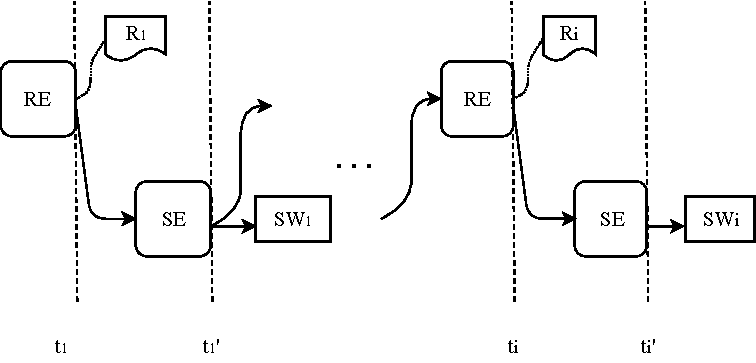
\includegraphics[width=0.9\textwidth]{C:/Users/chuprina/Documents/PhD/Conferences/git/RE/workshop_2018/IEEEtran/pictures/Metrics_shot.pdf}
	\caption{metrics explanation}
	\label{fig:Metrics_shot}
\end{figure}

\begin{figure}[!t]
	\centering
		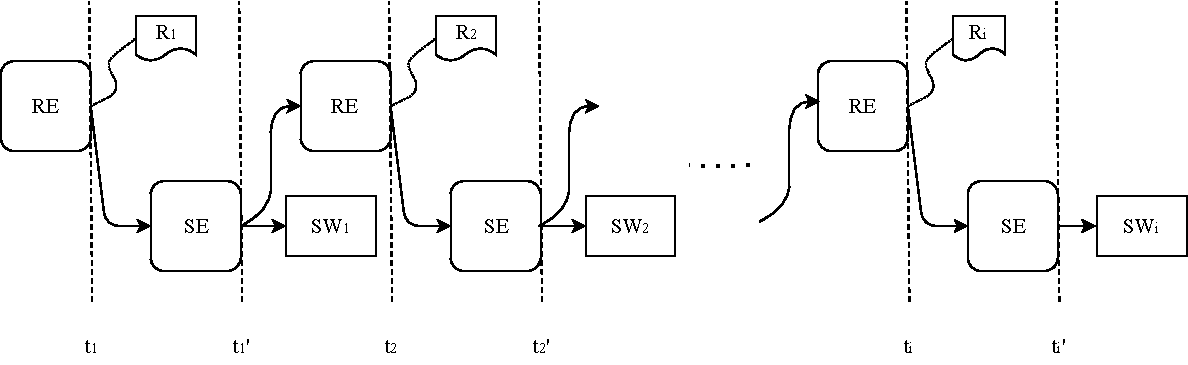
\includegraphics[width=0.9\textwidth]{C:/Users/chuprina/Documents/PhD/Conferences/git/RE/workshop_2018/IEEEtran/pictures/MetricsDiag.pdf}
	\caption{metrics explanation}
	\label{fig:Metrics_shot}
\end{figure}


$\mu_{1}(R_{j}) = i-j$

$\mu_{2}(R_{j}) = t_{i}-t_{j}$

$\mu_{3}(R_{j}) = \displaystyle\sum_{j} t_{j+1}-t_{j}\acute{}$

$\mu_{4} = \displaystyle\sum_{j} (t_{j+1}-t_{j}\acute{} + p_{j}*(t_{j}\acute{} - t_{j}))$


